\noindent\emph{Literature crosscheck (added post-vetting).} The campaign's lineage
crossmatch omitted the Huang+2020 DECaLS catalogue and did not query the wider
literature. A full check --- Huang+2020 plus a NED/SIMBAD cone search --- finds that
\textbf{five of these eight systems are previously-published lenses} (flagged
\emph{Known} below; mostly Huang+2020, one also in the SOAR Gravitational Arc
Survey). Only \texttt{s\_327526\_9059}, \texttt{s\_340971\_2860}, and
\texttt{s\_325163\_2981} are genuinely new (absent from the lineage \emph{and} the
literature). The recoveries are an external validation of the v3$+$cascade finder;
the net-new count here is \textbf{3}, not 8.\par\smallskip

\begin{figure}[ht]\centering
\begin{minipage}[b]{0.32\linewidth}\centering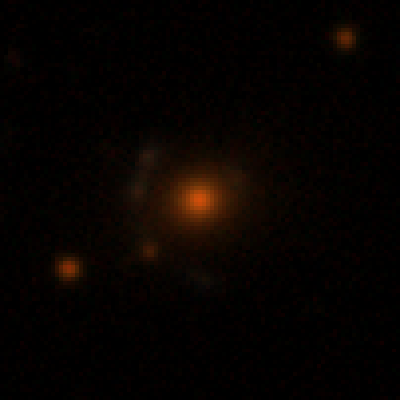
\includegraphics[width=\linewidth]{figures/cand_s_340513_3688_desi.png}\\[2pt]{\scriptsize DESI \emph{grz} (0.262\arcsec/px)}\end{minipage}\hfill
\begin{minipage}[b]{0.32\linewidth}\centering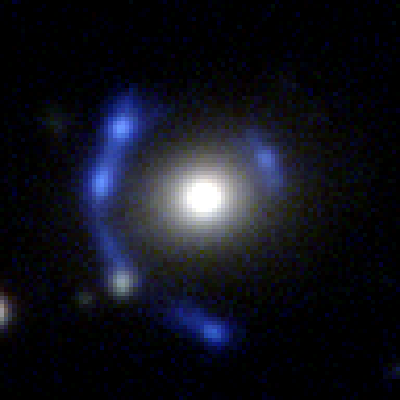
\includegraphics[width=\linewidth]{figures/cand_s_340513_3688_hsc.png}\\[2pt]{\scriptsize HSC \emph{grizy} (0.168\arcsec/px)}\end{minipage}\hfill
\begin{minipage}[b]{0.32\linewidth}\centering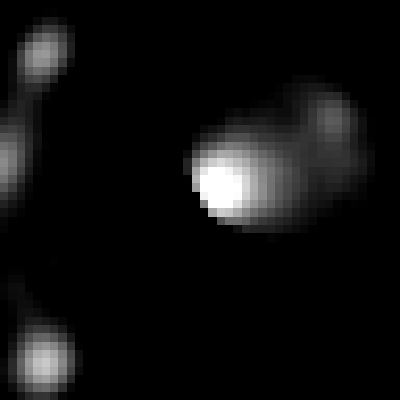
\includegraphics[width=\linewidth]{figures/cand_s_340513_3688_hscsub.png}\\[2pt]{\scriptsize HSC lens-light subtracted}\end{minipage}
\caption{\texttt{s\_340513\_3688} (RA 16.3319, Dec +1.7490) --- HSC tier-2 grade \textbf{A}, $p_{\rm lens}$ 0.22$\to$0.97, \vb{} 0.77. \emph{Known}: Huang+2020 \texttt{DESI-016.3319+01.7490} (grade A), $0.1\arcsec$.}
\end{figure}
\begin{figure}[ht]\centering
\begin{minipage}[b]{0.32\linewidth}\centering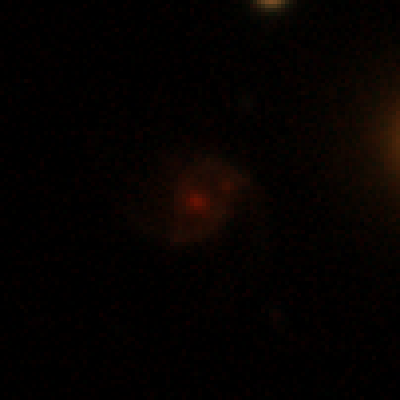
\includegraphics[width=\linewidth]{figures/cand_s_327526_9059_desi.png}\\[2pt]{\scriptsize DESI \emph{grz} (0.262\arcsec/px)}\end{minipage}\hfill
\begin{minipage}[b]{0.32\linewidth}\centering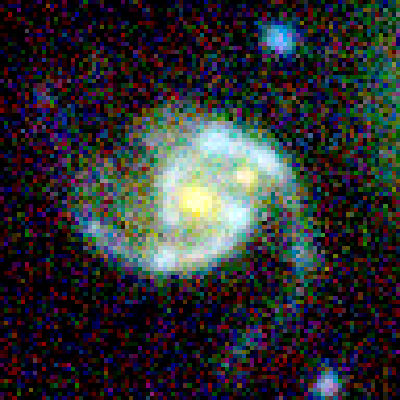
\includegraphics[width=\linewidth]{figures/cand_s_327526_9059_hsc.png}\\[2pt]{\scriptsize HSC \emph{grizy} (0.168\arcsec/px)}\end{minipage}\hfill
\begin{minipage}[b]{0.32\linewidth}\centering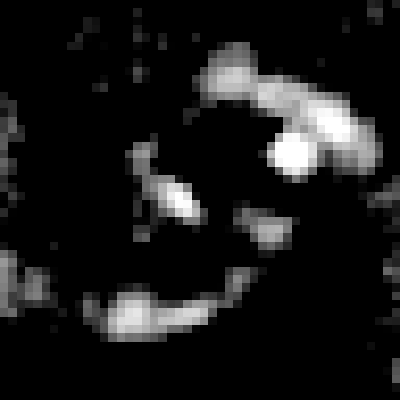
\includegraphics[width=\linewidth]{figures/cand_s_327526_9059_hscsub.png}\\[2pt]{\scriptsize HSC lens-light subtracted}\end{minipage}
\caption{\texttt{s\_327526\_9059} (RA 9.7222, Dec -0.4093) --- HSC tier-2 grade \textbf{A}, $p_{\rm lens}$ 0.04$\to$0.92, \vb{} 0.74. \emph{New}: absent from the lineage and from NED/SIMBAD.}
\end{figure}
\begin{figure}[ht]\centering
\begin{minipage}[b]{0.32\linewidth}\centering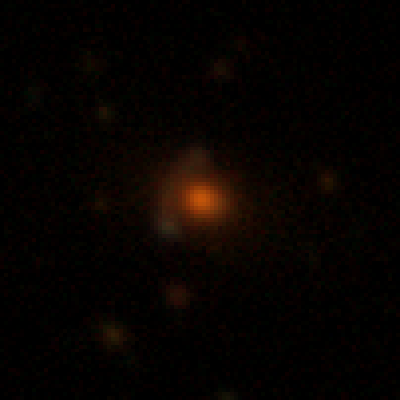
\includegraphics[width=\linewidth]{figures/cand_s_351303_461_desi.png}\\[2pt]{\scriptsize DESI \emph{grz} (0.262\arcsec/px)}\end{minipage}\hfill
\begin{minipage}[b]{0.32\linewidth}\centering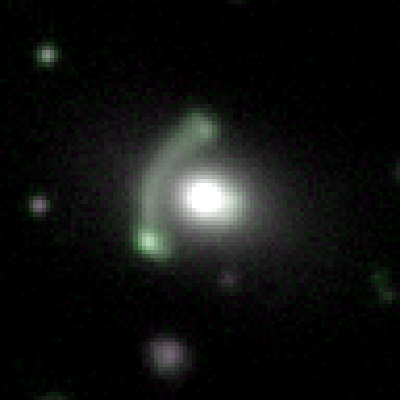
\includegraphics[width=\linewidth]{figures/cand_s_351303_461_hsc.png}\\[2pt]{\scriptsize HSC \emph{grizy} (0.168\arcsec/px)}\end{minipage}\hfill
\begin{minipage}[b]{0.32\linewidth}\centering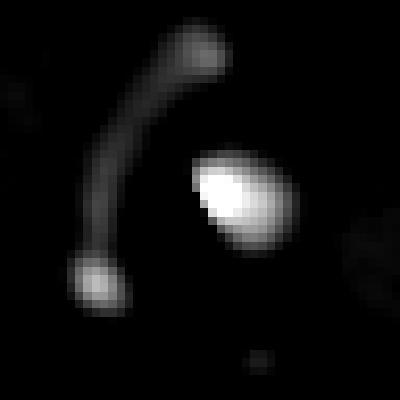
\includegraphics[width=\linewidth]{figures/cand_s_351303_461_hscsub.png}\\[2pt]{\scriptsize HSC lens-light subtracted}\end{minipage}
\caption{\texttt{s\_351303\_461} (RA 194.5345, Dec +3.5358) --- HSC tier-2 grade \textbf{A}, $p_{\rm lens}$ 0.62$\to$0.92, \vb{} 0.89. \emph{Known}: Huang+2020 \texttt{DESI-194.5344+03.5358} (grade A), $0.2\arcsec$.}
\end{figure}
\begin{figure}[ht]\centering
\begin{minipage}[b]{0.32\linewidth}\centering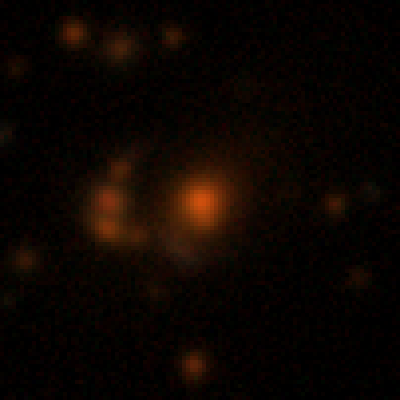
\includegraphics[width=\linewidth]{figures/cand_s_345385_1515_desi.png}\\[2pt]{\scriptsize DESI \emph{grz} (0.262\arcsec/px)}\end{minipage}\hfill
\begin{minipage}[b]{0.32\linewidth}\centering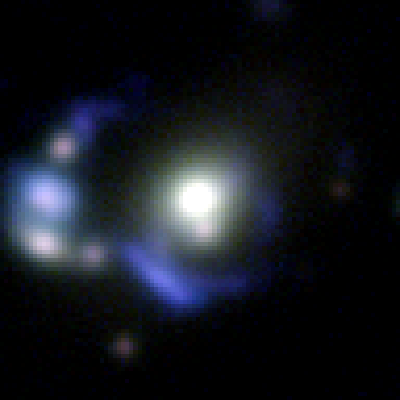
\includegraphics[width=\linewidth]{figures/cand_s_345385_1515_hsc.png}\\[2pt]{\scriptsize HSC \emph{grizy} (0.168\arcsec/px)}\end{minipage}\hfill
\begin{minipage}[b]{0.32\linewidth}\centering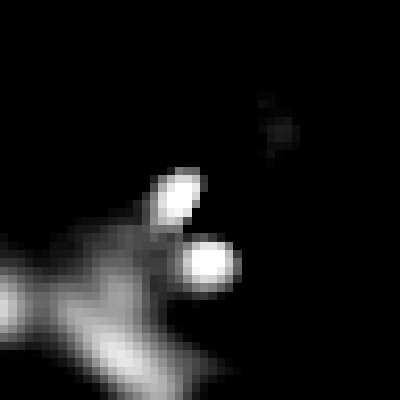
\includegraphics[width=\linewidth]{figures/cand_s_345385_1515_hscsub.png}\\[2pt]{\scriptsize HSC lens-light subtracted}\end{minipage}
\caption{\texttt{s\_345385\_1515} (RA 154.3116, Dec +2.4885) --- HSC tier-2 grade \textbf{A}, $p_{\rm lens}$ 0.10$\to$0.92, \vb{} 0.81. \emph{Known}: Huang+2020 \texttt{DESI-154.3116+02.4885} (grade C), $0.1\arcsec$. (= 8th detection s\_345385\_1514, the adjacent $\sim$1\arcsec\ pair, omitted)}
\end{figure}
\begin{figure}[ht]\centering
\begin{minipage}[b]{0.32\linewidth}\centering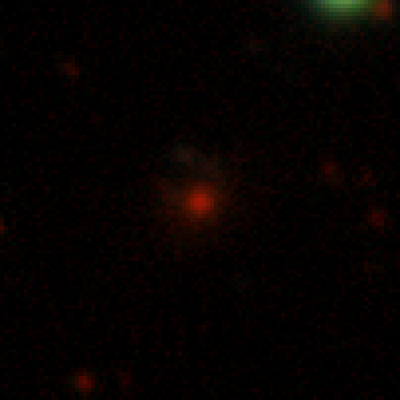
\includegraphics[width=\linewidth]{figures/cand_s_340971_2860_desi.png}\\[2pt]{\scriptsize DESI \emph{grz} (0.262\arcsec/px)}\end{minipage}\hfill
\begin{minipage}[b]{0.32\linewidth}\centering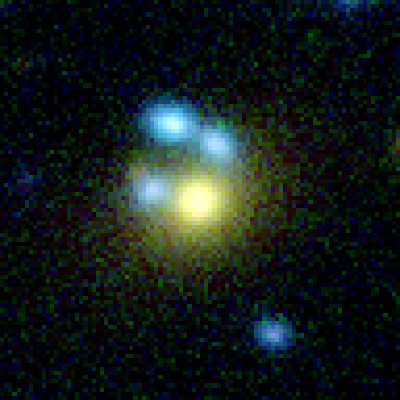
\includegraphics[width=\linewidth]{figures/cand_s_340971_2860_hsc.png}\\[2pt]{\scriptsize HSC \emph{grizy} (0.168\arcsec/px)}\end{minipage}\hfill
\begin{minipage}[b]{0.32\linewidth}\centering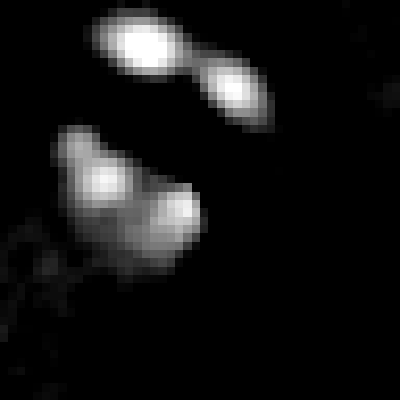
\includegraphics[width=\linewidth]{figures/cand_s_340971_2860_hscsub.png}\\[2pt]{\scriptsize HSC lens-light subtracted}\end{minipage}
\caption{\texttt{s\_340971\_2860} (RA 130.8571, Dec +1.7840) --- HSC tier-2 grade \textbf{A}, $p_{\rm lens}$ 0.12$\to$0.91, \vb{} 0.76. \emph{New}: absent from the lineage and from NED/SIMBAD.}
\end{figure}
\begin{figure}[ht]\centering
\begin{minipage}[b]{0.32\linewidth}\centering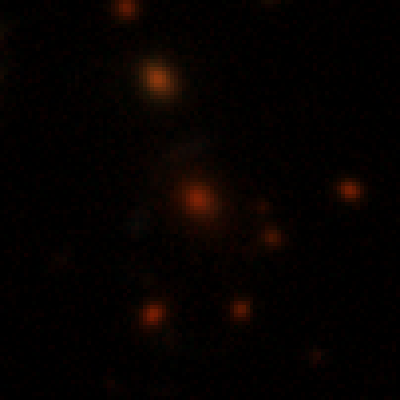
\includegraphics[width=\linewidth]{figures/cand_s_326089_1785_desi.png}\\[2pt]{\scriptsize DESI \emph{grz} (0.262\arcsec/px)}\end{minipage}\hfill
\begin{minipage}[b]{0.32\linewidth}\centering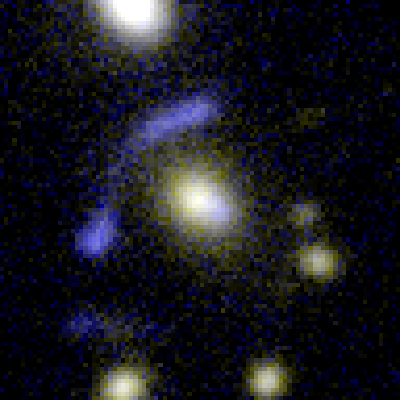
\includegraphics[width=\linewidth]{figures/cand_s_326089_1785_hsc.png}\\[2pt]{\scriptsize HSC \emph{grizy} (0.168\arcsec/px)}\end{minipage}\hfill
\begin{minipage}[b]{0.32\linewidth}\centering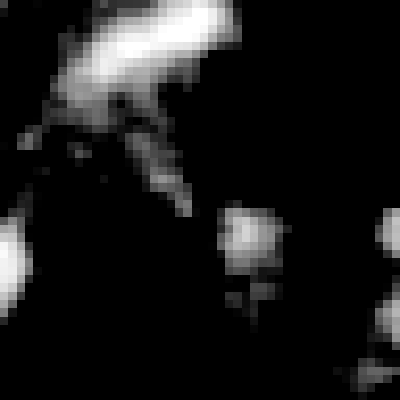
\includegraphics[width=\linewidth]{figures/cand_s_326089_1785_hscsub.png}\\[2pt]{\scriptsize HSC lens-light subtracted}\end{minipage}
\caption{\texttt{s\_326089\_1785} (RA 10.2876, Dec -0.7303) --- HSC tier-2 grade \textbf{A}, $p_{\rm lens}$ 0.03$\to$0.82, \vb{} 0.83. \emph{Known}: Huang+2020 \texttt{DESI-010.2876-00.7303} (grade B), also SOGRAS~J0041$-$0043, $0.1\arcsec$.}
\end{figure}
\begin{figure}[ht]\centering
\begin{minipage}[b]{0.32\linewidth}\centering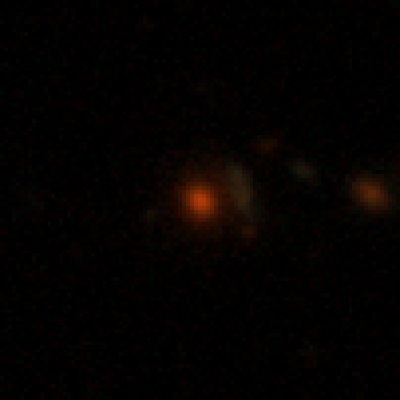
\includegraphics[width=\linewidth]{figures/cand_s_325163_2981_desi.png}\\[2pt]{\scriptsize DESI \emph{grz} (0.262\arcsec/px)}\end{minipage}\hfill
\begin{minipage}[b]{0.32\linewidth}\centering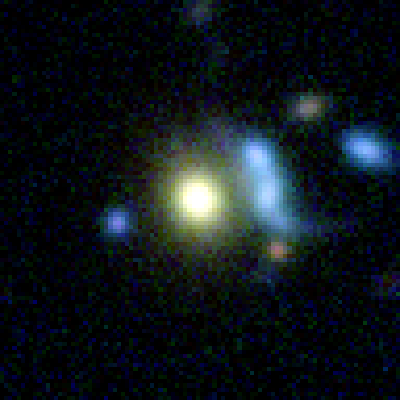
\includegraphics[width=\linewidth]{figures/cand_s_325163_2981_hsc.png}\\[2pt]{\scriptsize HSC \emph{grizy} (0.168\arcsec/px)}\end{minipage}\hfill
\begin{minipage}[b]{0.32\linewidth}\centering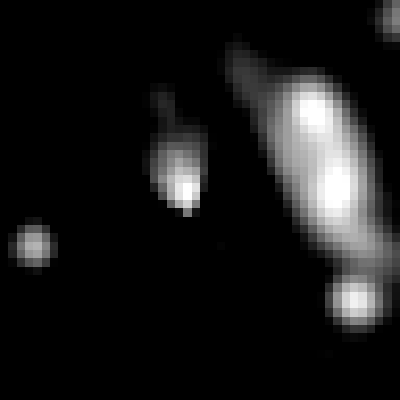
\includegraphics[width=\linewidth]{figures/cand_s_325163_2981_hscsub.png}\\[2pt]{\scriptsize HSC lens-light subtracted}\end{minipage}
\caption{\texttt{s\_325163\_2981} (RA 138.8482, Dec -0.9226) --- HSC tier-2 grade \textbf{A}, $p_{\rm lens}$ 0.18$\to$0.82, \vb{} 0.74. \emph{New}: absent from the lineage and from NED/SIMBAD.}
\end{figure}
\begin{figure}[ht]\centering
\begin{minipage}[b]{0.32\linewidth}\centering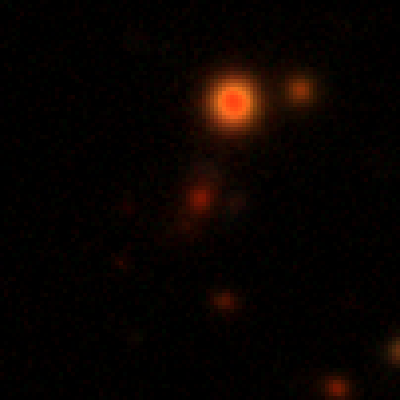
\includegraphics[width=\linewidth]{figures/cand_s_318043_1037_desi.png}\\[2pt]{\scriptsize DESI \emph{grz} (0.262\arcsec/px)}\end{minipage}\hfill
\begin{minipage}[b]{0.32\linewidth}\centering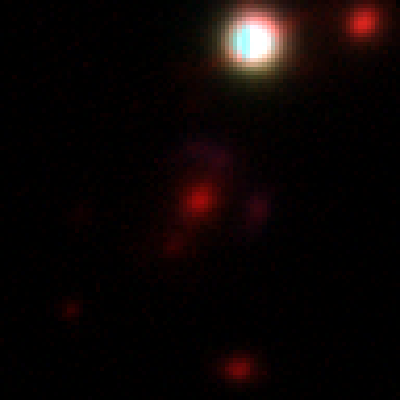
\includegraphics[width=\linewidth]{figures/cand_s_318043_1037_hsc.png}\\[2pt]{\scriptsize HSC \emph{grizy} (0.168\arcsec/px)}\end{minipage}\hfill
\begin{minipage}[b]{0.32\linewidth}\centering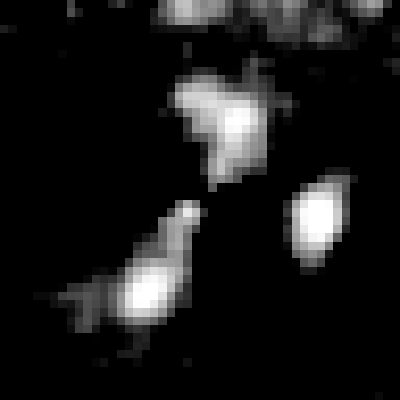
\includegraphics[width=\linewidth]{figures/cand_s_318043_1037_hscsub.png}\\[2pt]{\scriptsize HSC lens-light subtracted}\end{minipage}
\caption{\texttt{s\_318043\_1037} (RA 158.7893, Dec -2.3037) --- HSC tier-2 grade \textbf{B}, $p_{\rm lens}$ 0.04$\to$0.45, \vb{} 0.86. \emph{Known}: Huang+2020 \texttt{DESI-158.7893-02.3037} (grade B), $0.1\arcsec$.}
\end{figure}
